\section{Motivation}
\subsection{The physics}
\begin{frame}{}{}
	\begin{columns}
	 	\column{.3\textwidth}
	 		\begin{center} 
				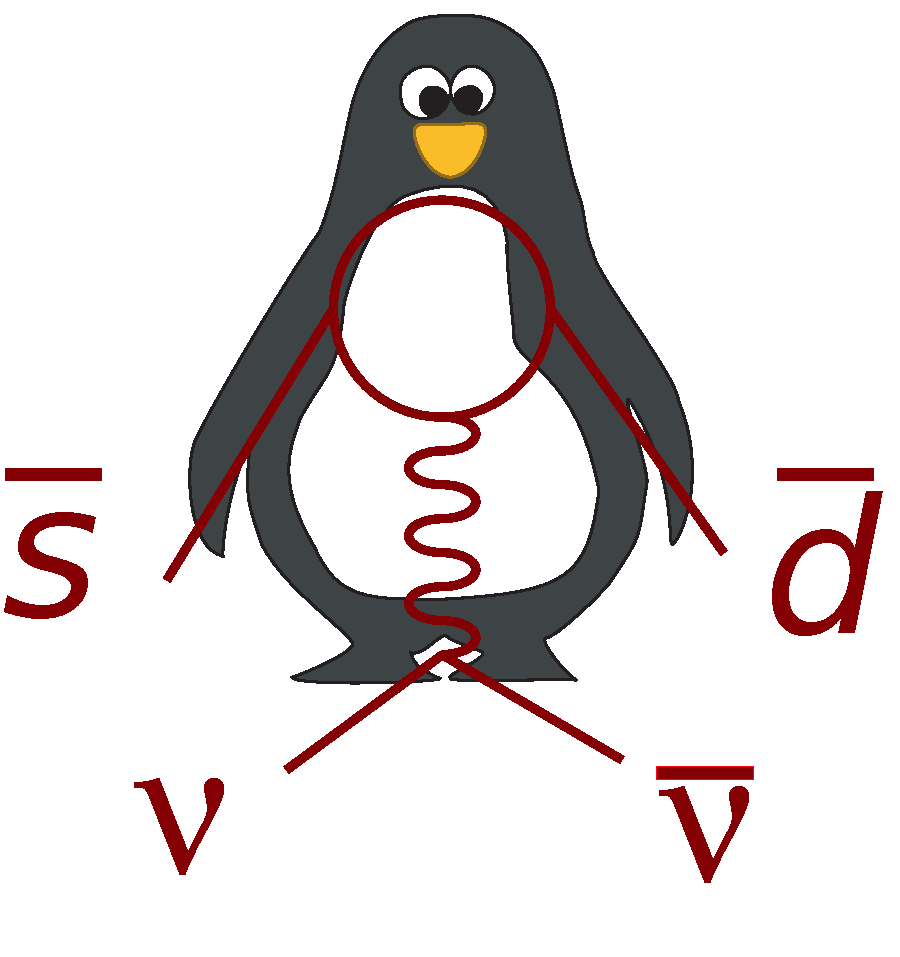
\includegraphics[height=4cm]{penguino}
			\end{center}
	    \column{.65	\textwidth}
	    	\begin{block}{$K^+ \rightarrow \pi^+ \nu \bar{\nu} ~\Leftrightarrow ~
	    	V_{td}$ of CKM matrix} SM branching ratio: $(8.5\pm 0.7)\cdot 10^{-11}$
			\end{block}
			\begin{block}{Measurement from BNL (Brookhaven)}
				The only experimental data so far (7 candidates)
	    		E787 and E949:\\
	    		$BR(K^+ \rightarrow \pi^+ \nu \bar{\nu})=(17.3^{+11.5}_{-10.5})\cdot
	    		10^{-11}$
			\end{block}
			\begin{exampleblock}{NA62 aims $\sigma < 10\%$ with 100 events}
	    		$\approx 10^{13} ~ K^+$ decays required
			\end{exampleblock}
	\end{columns}
	\begin{block}{High efficiency needed $\Rightarrow$ high data rate}
		Signal-to-noise ratio of 1/10 planned with an event rate of 10 MHz
	\end{block}
\end{frame}

\begin{frame}{Background channels to be suppressed by the detector}{}
	\begin{align*}
	   K^+ &\rightarrow \mu^+ \nu &(63\%) &\rightarrow \mu \text{ veto} \\
		 K^+ &\rightarrow \pi^+ \pi^0 &(21\%) &\rightarrow \gamma \text{ veto} \\
	  	 K^+ &\rightarrow \pi^+ \pi^+ \pi^- &(6\%) &\rightarrow \text{charged particle veto} \\
	  	 K^+ &\rightarrow \pi^0 e^+ \nu &(5\%) &\rightarrow \gamma \text{ veto}  \\
	  	  K^+ &\rightarrow \pi^0 \mu^+ \nu &(3\%) &\rightarrow \gamma, \mu \text{ veto} \\
	  	   K^+ &\rightarrow \pi^+ \pi^0 \pi^0 &(2\%) &\rightarrow \gamma \text{
	  	  veto}		  	
	\end{align*}
	\begin{ergo}
		Detector dominated by vetos
	\end{ergo}
\end{frame}

\section{The experiment}
\subsection{Subdetectors}
\begin{frame}{Experiment overview}{}
	\begin{center} 
		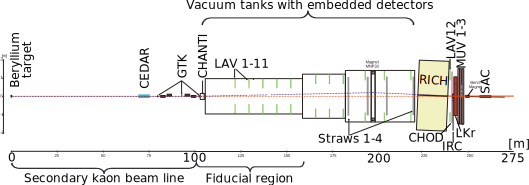
\includegraphics[width=\textwidth]{na62-overview}
	\end{center}
\end{frame}

\begin{frame}{CEDAR}{}
	\begin{center} 
		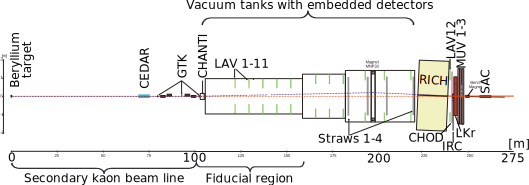
\includegraphics[width=\textwidth]{na62-overview}
	\end{center}
	\begin{block}{Differential Cerenkov counter}
		$K^+$ identification \\
		Mirrors collect $K^+$-specific Cerenkov light
	\end{block}
\end{frame}

\begin{frame}{GTK}{}
	\begin{center} 
		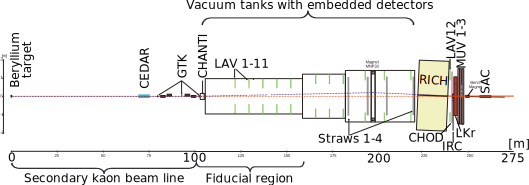
\includegraphics[width=\textwidth]{na62-overview}
	\end{center}
	\begin{block}{Gigatracker (second Achromat)}
		Timing, momentum and angle of all particles using silicon pixels \\
		750 MHz event rate!!!
	\end{block}
\end{frame}

\begin{frame}{Straws}{}
	\begin{center} 
		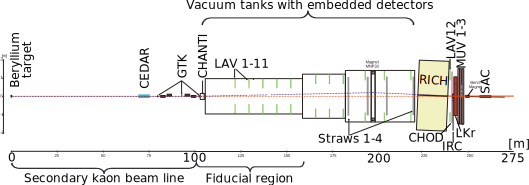
\includegraphics[width=\textwidth]{na62-overview}
	\end{center}
	\begin{block}{Spectrometer}
		Tracking of charged particles within a magnetic field
	\end{block}
\end{frame}

\begin{frame}{Photon vetos part 1: LAV, IRC, SAC}{}
	\begin{center} 
		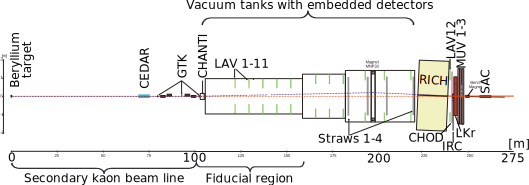
\includegraphics[width=\textwidth]{na62-overview}
	\end{center}
	\begin{block}{Photon vetos}
		Huge range of angle to be covered \\ 
		Scintillators at different positions (lead-glass reused from OPAL)
	\end{block}
\end{frame}

\begin{frame}{Photon veto part 2: LKr}{}
	\begin{center} 
		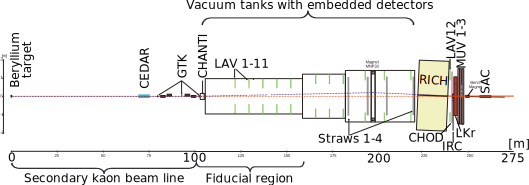
\includegraphics[width=\textwidth]{na62-overview}
	\end{center}
	\begin{block}{Liquid Krypton calorimeter}
		Photon veto for central angles range\\
		Muon veto \\
		Reused from NA48 $\Rightarrow$ can be used as calorimeter for analysis of
		additional rare decays
	\end{block}
\end{frame}

\begin{frame}{Rich}{}
	\begin{center} 
		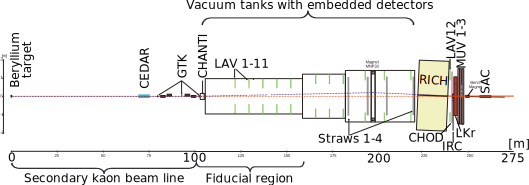
\includegraphics[width=\textwidth]{na62-overview}
	\end{center}
	\begin{block}{Ring Imaging Cherenkov}
		Separate $\pi^+$ from $\mu^+$ between 15 and 35 GeV/c (L0 trigger)
	\end{block}
\end{frame}



\begin{frame}{MUV}{}
	\begin{center} 
		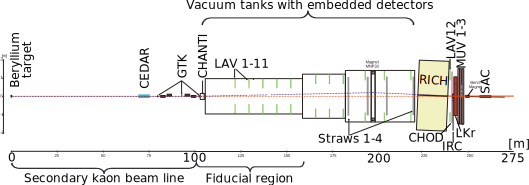
\includegraphics[width=\textwidth]{na62-overview}
	\end{center}
	\begin{block}{Muon veto}
		Scintillator-iron-sandwich mainly produced in Mainz 
	\end{block}
\end{frame}

% \begin{frame}{Subdetector functionalities}{}
% \begin{description}
%   \item[CEDAR] Differential Cerenkov counter for Kaon tagging
%   \item[GTK] Timing, momentum, angle of all hadrons
%   \item[CHANTI] Detect inelastic interactions in GTK ($K^+ \rightarrow \pi^+
%   \pi^0$)
%     \item[LAV] Large angle photon veto
%     \item[LKr] Medium angle photon veto
%     \item[IRC \& SAC] Small angle photon veto  
%    	\item[STRAW] Direction and momentum of charged particles
%    	\item[RICH] Ring Imaging Cherenkov for vetoing muons
%    	\item[CHOD] Charged hodoscope for low energy hadrons from photonuclear
%    	interactions
%    	\item[MUV] Muon Veto
% \end{description}
% \end{frame}

\begin{frame}{Data rates}{}
	\begin{center}
		\textbf{10 MHz unsteady $K^+$ rate}
	\end{center}
	\begin{table}[H]
		\begin{center}
			\begin{tabular}{c|c|>{\centering\arraybackslash}m{3cm}}
			Detector	&	Event size [B] &	Data rate [GBps]\\
			\hline
			CEDAR	&	216		&	2.16	\\
			GTK 	&	2250	&	22.50 	\\
			CHANTI	&	192		&	1.92 	\\
			LAV 	&	160		&	1.60 	\\
			STRAW 	&	768		&	7.68 	\\
			RICH 	&	160		&	1.60 	\\
			CHOD	&	$\ll1000$	&	$\ll10$\\
			MUV 	&	768		&	7.68 \\
			IRC \& SAC 	& 576	& 	5.76 	\\
			\textbf{LKR}		&	\textbf{222~k}	&	\textbf{2220}	\\
			\hline
			\textbf{Sum}	&	\textbf{$\approx$227~kB}	&	\textbf{$\approx$2.3~TBps}\\
			\end{tabular}
		\end{center}
	\end{table}
\end{frame}